\section{Технологический раздел \hfill}
\vspace{\baselineskip}

\subsection{Требования к программному обеспечению}

Программа должна предоставлять следующие возможности:
\begin{itemize}[label=---]
    \item выбор режима обработки данных (линейный или конвейерный);
    \item ввод размера графа и количества графов;
    \item измерение времени обработки каждой задачи на каждом из этапов;
    \item вывод результата в файл с расширением dot.
\end{itemize}

\subsection{Средства реализации}

В качестве языка программирования для реализации лабораторной работы был выбран язык C++ \cite{cpp}. Данный язык предоставляет необходимые библиотеки для работы с нативными потоками. 

Для визуализации данных эксперимента был выбран язык программирования Python \cite{python}, так как он предоставляет большое число настроек параметров графика с использованием простого синтаксиса. 

Для замера процессорного времени использовалась функция библиотеки chrono \cite{chrono} \texttt{std::chrono::system\_clock::now()}.

\subsection{Используемые структуры данных}

В программе используется структура graph\_t, описанная в листинге \ref{lst:graph_t}. Ее полями являются размер графа, матрица со значениями 0 и 1 в зависимости от наличия ребра между вершинами $i$ и $j$, массив с количеством смежных вершин для каждой вершины, описание графа в формате graphviz.

\clearpage

\begin{lstlisting}[label=lst:graph_t, caption=Структура graph\_t]
struct graph_t
{
    int size;
    int **matrix;
    int *neighbors_num;
    std::vector<std::string> description;
};
\end{lstlisting}

\subsection{Реализации алгоритмов}
В листингах \ref{lst:count_neighbors}-\ref{lst:write_to_file} представлены реализации этапов алгоритма раскраски графа по количеству смежных вершин. 

В листинге \ref{lst:linear} приведена реализация линейного алгоритма раскраски графа по количеству смежных вершин.

В листингах \ref{lst:parallel} представлена реализация алгоритма раскраски графа с использованием конвейерных вычислений. 

\clearpage

\begin{lstlisting}[label=lst:count_neighbors, caption=Этап вычисления числа соседей каждого узла]
void count_neighbors(graph_t &graph)
{
    for (int i = 0; i < graph.size; i++)
    {
        int str_sum = 0;
        for (int j = 0; j < graph.size; j++)
            str_sum += graph.matrix[i][j];
        graph.neighbors_num[i] = str_sum;
    }
}
\end{lstlisting}

\begin{lstlisting}[label=lst:make_description, caption=Этап составления описания графа для graphviz]
void make_description(graph_t &graph)
{
    for (int i = 0; i < graph.size; i++)
    {
        double color = double(graph.neighbors_num[i]) / 
                       graph.size * 0.4 + 0.6;

        graph.description.push_back("\t" + std::to_string(i+1) 
              + [style=\"filled\", fillcolor=\"" + 
              std::to_string(color) + " 1.000 1.000\"]; \n");
        
        for (int j = i + 1; j < graph.size; j++)
        {
            if (graph.matrix[i][j] == 1)
                graph.description.push_back("\t" + std::to_string
                (i+1) + " -- " + std::to_string(j+1) + ";\n");
        }
    }
}
\end{lstlisting}
\clearpage

\begin{lstlisting}[label=lst:write_to_file, caption=Этап вывода описания графа в файл с расширением dot]
void write_to_file(graph_t &graph, int num)
{
    FILE *file = fopen(("output" + std::to_string(num) + ".dot").c_str(), "w");

    fprintf(file, "graph { \n");

    for (int i = 0; i < graph.description.size(); i++)
    {
        fprintf(file, graph.description[i].c_str());
    }

    fprintf(file, "}\n");

    fclose(file);
}
\end{lstlisting}

\clearpage

\begin{lstlisting}[label=lst:linear, caption=Реализация линейного алгоритма]
void stage1_linear(graph_t &graph, int task_num)
{
    count_neighbors(graph);
}

void stage2_linear(graph_t &graph, int task_num)
{   
    make_description(graph);
}

void stage3_linear(graph_t &graph, int task_num)
{   
    write_to_file(graph, task_num);
}

void parse_linear(int count, size_t size)
{
    std::queue<graph_t> q1, q2, q3;
    queues_t queues = {.q1 = q1, .q2 = q2, .q3 = q3};

    for (int i = 0; i < count; i++)
    {
        graph_t res = generate_graph(size);
        queues.q1.push(res);
    }

    for (int i = 0; i < count; i++)
    {
        graph_t graph = queues.q1.front();
        stage1_linear(graph, i + 1);
        queues.q1.pop();
        queues.q2.push(graph);

        graph = queues.q2.front();
        stage2_linear(graph, i + 1);
        queues.q2.pop();
        queues.q3.push(graph);

        graph = queues.q3.front();
        stage3_linear(graph, i + 1);
        queues.q3.pop();
    }
}
\end{lstlisting}
\clearpage

\begin{lstlisting}[label=lst:parallel, caption=Реализация вычислительного конвейера]
void stage1_parallel(std::queue<graph_t> &q1, 
    std::queue<graph_t> &q2, std::queue<graph_t> &q3)
{
    int task_num = 1;

    std::mutex m;

    while(!q1.empty())
    {      
        m.lock();
        graph_t graph = q1.front();
        m.unlock();

        count_neighbors(graph);

        m.lock();
        q2.push(graph);
        q1.pop();
        m.unlock();
    }
}

void stage2_parallel(std::queue<graph_t> &q1, 
     std::queue<graph_t> &q2, std::queue<graph_t> &q3)
{
    int task_num = 1;

    std::mutex m;

    do
    {   
        m.lock();
        bool is_q2empty = q2.empty();
        m.unlock();

        if (!is_q2empty)
        {   
            m.lock();
            graph_t graph = q2.front();
            m.unlock();

            make_description(graph);

            m.lock();
            q3.push(graph);
            q2.pop();
            m.unlock();
        }
    } while (!q1.empty() || !q2.empty());
}

void stage3_parallel(std::queue<graph_t> &q1, 
    std::queue<graph_t> &q2, std::queue<graph_t> &q3)
{
    int task_num = 1;

    std::mutex m;

    do
    {
        m.lock();
        bool is_q3empty = q3.empty();
        m.unlock();

        if (!is_q3empty)
        {
            m.lock();
            graph_t graph = q3.front(); 
            m.unlock();

            write_to_file(graph, task_num++);

            m.lock();
            q3.pop();
            m.unlock();
        }
    } while (!q1.empty() || !q2.empty() || !q3.empty());
}

void parse_parallel(int count, size_t size)
{
    std::queue<graph_t> q1, q2, q3;
    queues_t queues = {.q1 = q1, .q2 = q2, .q3 = q3};

    for (int i = 0; i < count; i++)
    {
        graph_t res = generate_graph(size);
        q1.push(res);
    }

    std::thread threads[THREADS];

    threads[0] = std::thread(stage1_parallel, 
            std::ref(q1), std::ref(q2), std::ref(q3));
    threads[1] = std::thread(stage2_parallel, 
            std::ref(q1), std::ref(q2), std::ref(q3));
    threads[2] = std::thread(stage3_parallel, 
            std::ref(q1), std::ref(q2), std::ref(q3));

    for (int i = 0; i < THREADS; i++)
        threads[i].join();
}
\end{lstlisting}

\clearpage

\subsection{Тестирование}

На рисунке \ref{fig:test1_in} приведен пример исходного графа. На рисунке \ref{fig:test1_out} -- ожидаемый результат закраски по количеству смежных вершин для этого графа. Тест пройден успешно.

\begin{figure}[h!btp]
	\centering
	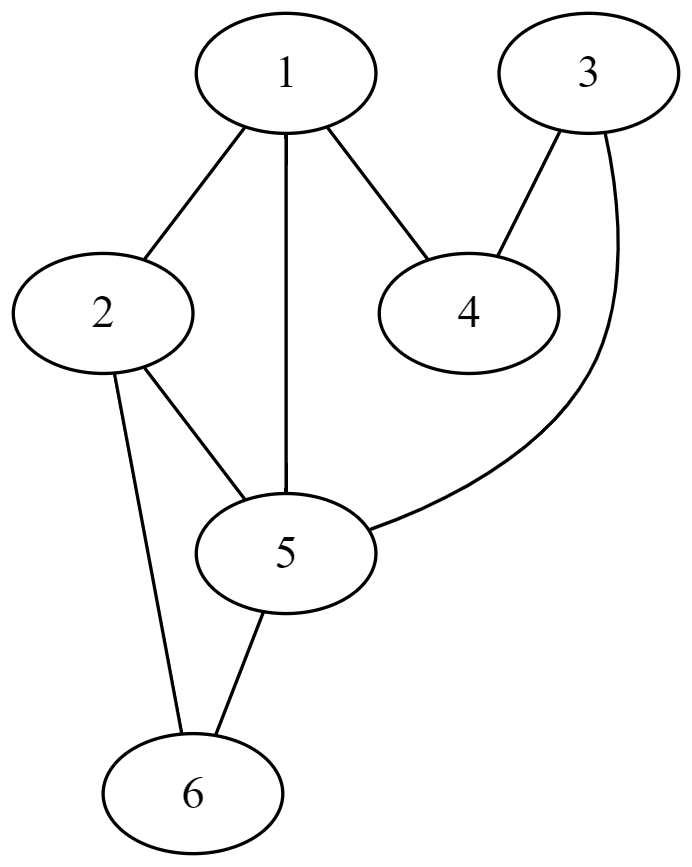
\includegraphics[width=200pt]{inc/test1_in.png}
	\caption{Исходный граф}
	\label{fig:test1_in}	
\end{figure}

\begin{figure}[h!btp]
	\centering
	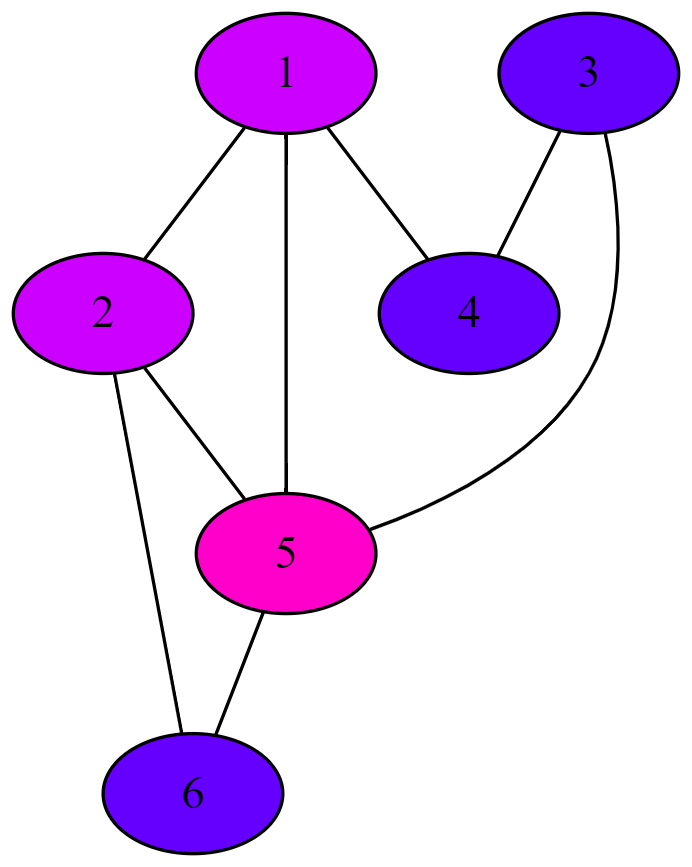
\includegraphics[width=200pt]{inc/test1_out.png}
	\caption{Ожидаемый результат закраски графа}
	\label{fig:test1_out}	
\end{figure}

\subsection*{Вывод}

Были описаны требования к программному обеспечению, средства реализации, приведены реализации алгоритмов и тест, успешно пройденный программой.
